\section{Micro-CUDA Compiler (\texttt{ucuda-cc})}

To enable rapid kernel development, we developed \texttt{ucuda-cc}, a custom compiler that translates a C-like high-level language into optimized Micro-CUDA assembly. The compiler is implemented in Python to ensure portability and easy integration with the host CLI.

\subsection{Compiler Architecture}
The compiler infrastructure leverages the industry-standard LLVM framework to ensure robustness and extensibility. As illustrated in Figure \ref{fig:compiler_arch}, the pipeline consists of a modular transformation flow:

\begin{enumerate}
    \item \textbf{Frontend (Clang)}: We utilize Clang to assist in parsing standard CUDA-like C++ code, performing syntax checking, and generating machine-independent LLVM Intermediate Representation (IR).
    \item \textbf{Middle-end (LLVM OPT)}: Standard optimization passes (e.g., constant propagation, dead code elimination, loop unrolling) are applied to the IR.
    \item \textbf{Backend (MCC)}: Our custom Python-based backend (\texttt{mcc.py}) consumes the optimized LLVM IR. It performs two key tasks:
    \begin{itemize}
        \item \textbf{Instruction Selection}: Mapping generic IR instructions to the specific Micro-CUDA ISA (e.g., \texttt{fadd} $\to$ \texttt{FADD}).
        \item \textbf{Register Allocation}: Mapping infinite virtual registers to the fixed 32 physical registers per lane using a linear scan algorithm.
    \end{itemize}
\end{enumerate}

\begin{figure}[htbp]
\centering
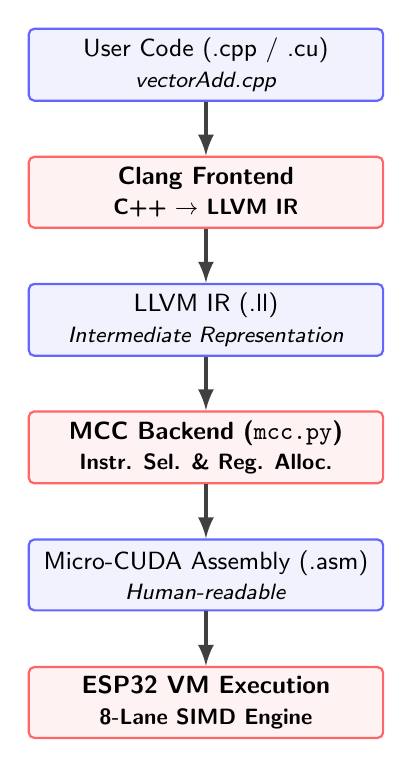
\begin{tikzpicture}[
    scale=0.9,
    node distance=1.5cm,
    data_node/.style={
        rectangle,
        draw=blue!60,
        fill=blue!5,
        thick,
        rounded corners=2pt,
        minimum width=4.5cm,
        minimum height=0.9cm,
        align=center,
        font=\small\sffamily
    },
    proc_node/.style={
        rectangle,
        draw=red!60,
        fill=red!5,
        thick,
        rounded corners=2pt,
        minimum width=4.5cm,
        minimum height=0.9cm,
        align=center,
        font=\small\bfseries\sffamily
    },
    arrow/.style={->, ultra thick, -latex, darkgray}
]

    % Nodes with manual positioning for stability
    \node[data_node] (src) at (0, 0) {User Code (.cpp / .cu)\\ \footnotesize \textit{vectorAdd.cpp}};
    
    \node[proc_node] (clang) at (0, -1.8) {Clang Frontend\\ \footnotesize C++ $\to$ LLVM IR};
    
    \node[data_node] (ir) at (0, -3.6) {LLVM IR (.ll)\\ \footnotesize \textit{Intermediate Representation}};
    
    \node[proc_node] (mcc) at (0, -5.4) {MCC Backend (\texttt{mcc.py})\\ \footnotesize Instr. Sel. \& Reg. Alloc.};
    
    \node[data_node] (asm) at (0, -7.2) {Micro-CUDA Assembly (.asm)\\ \footnotesize \textit{Human-readable}};
    
    \node[proc_node] (vm) at (0, -9.0) {ESP32 VM Execution\\ \footnotesize 8-Lane SIMD Engine};

    % Arrows
    \draw[arrow] (src) -- (clang);
    \draw[arrow] (clang) -- (ir);
    \draw[arrow] (ir) -- (mcc);
    \draw[arrow] (mcc) -- (asm);
    \draw[arrow] (asm) -- (vm);

\end{tikzpicture}
\caption{Micro-CUDA Compiler Workflow: Leveraging Clang/LLVM for robust code generation.}
\label{fig:compiler_arch}
\end{figure}

\subsection{Instruction Selection \& Mapping}
The backend (\texttt{MicroCUDABackend}) implements a direct mapping strategy from LLVM IR to Micro-CUDA ISA. Key translations include:

\begin{itemize}
    \item \textbf{Arithmetic}: LLVM \texttt{add/sub/mul} are mapped to \texttt{IADD/ISUB/IMUL}. Immediate operands are handled by loading constants into temporary registers via an 8-bit split-load sequence (\texttt{MOV+SHL+OR}) if they exceed the immediate field size.
    \item \textbf{Memory Access}: \texttt{getelementptr} instructions are lowered into explicit address calculations. The \texttt{LDX/STX} (Load/Store Indexed) instructions are used for gathered access, where the address is computed as $Base + Offset$.
    \item \textbf{Control Flow}: Vector comparisons (\texttt{icmp}) translate to predicate generation (\texttt{ISETP}). Branch instructions (\texttt{br}) are converted to \texttt{BRZ} (Branch if Zero) acting on the predicate register $P0$.
\end{itemize}

\subsection{Implementation: Regex-Based Frontend}
To maintain a lightweight footprint without requiring a full LLVM library link, the compiler utilizes a Python-based regex parser (\texttt{LLVMIRParser}). It scans the text-based \texttt{.ll} output from Clang, reconstructing the Control Flow Graph (CFG) and basic blocks.

\begin{lstlisting}[language=Python, caption={IR Parsing Logic (mcc.py)}]
# Extract function definitions
if line.startswith('define'):
    match = re.search(r'@(\w+)\(', line)
    current_func = match.group(1)

# Parse arithmetic instructions
elif re.match(r'%\w+\s*=\s*add', ir_inst):
    # logic to allocate registers and emit IADD...
\end{lstlisting}

\subsection{Register Allocation Strategy}
The \texttt{RegisterAllocator} class implements a greedy Linear Scan algorithm optimized for the 32-register constraint:
\begin{enumerate}
    \item \textbf{Liveness Tracking}: Variables are tracked from definition to last use.
    \item \textbf{Free Pool}: Freed registers are returned to a pool and reused for subsequent instructions to minimize pressure.
    \item \textbf{Constant Caching}: Frequently used constants are cached in registers to reduce code size overhead from repeated loads.
\end{enumerate}

\subsection{Integration with Host CLI}
\texttt{ucuda-cc} is integrated directly into the Python host environment, allowing for JIT-like compilation of kernels before upload.

\subsection{Usage \& API Reference}
The compiler exposes both a command-line interface (CLI) for batch processing and a Python API for dynamic runtime generation.

\subsubsection{Command-Line Interface}
Development follows a standard workflow similar to \texttt{nvcc}. The toolchain supports multiple hardware targets (e.g., standard ESP32 vs. ESP32-S3 with 8MB PSRAM).

\begin{lstlisting}[language=bash, caption={Compiling a kernel from the CLI}]
# Compile for ESP32-S3 (8MB PSRAM)
python compile_kernel.py vector_add.cu \
    --target esp32s3 \
    --output vector_add.asm

# View generated assembly with hardware header
cat vector_add.asm
\end{lstlisting}

\subsubsection{Python Dynamic API}
For seamless integration into AI frameworks (e.g., PyTorch-like workflows), the \texttt{compile\_kernel} function allows in-memory compilation.

\begin{lstlisting}[language=Python, caption={Dynamic Compilation API}]
from micro_cuda_compiler import compile_kernel

kernel_src = """
#include "mcuda.h"
__global__ void scale(int* data, int factor) {
    int idx = laneId();
    data[idx] *= factor;
}
"""

# Compile to Assembly (returns path)
_, asm_path = compile_kernel(
    kernel_src,
    target="esp32s3",
    output_asm="temp_scale.asm"
)

# Load into VM
loader.load_assembly(asm_path)
\end{lstlisting}

\subsubsection{Target Configurations}
The compiler validates hardware constraints based on the selected target:
\begin{itemize}
    \item \textbf{esp32}: Standard model (32KB VRAM, No PSRAM).
    \item \textbf{esp32s3}: AI-focused model (1MB VRAM, 8MB PSRAM).
\end{itemize}

